\documentclass[a4paper,8pt,openany]{book}
\usepackage[utf8]{inputenc}
\usepackage[french]{babel}
\usepackage[T1]{fontenc}
\usepackage{graphicx}
\usepackage{titlesec}
\usepackage{amsmath}
\usepackage{amsfonts}
\usepackage{comment}

\titleformat{\chapter}[block]
  {\normalfont\Huge\bfseries}% font of number
  {\chaptertitlename\ \thechapter~:}% format of number
  {20pt}% space between number and title
  {\Huge}% font of title

\titlespacing*{\chapter}
  {0pt}%  indent
  {0pt}% space before
  {20pt}% space after
\titlespacing*{\section}
  {0pt}%  indent
  {3.5ex plus 1ex minus .2ex}% space before
  {2.3ex plus .2ex}% space after

\newcommand\tab[1][1cm]{\hspace*{#1}}

\author{Mendy Fatnassi}
\title{Probabilite et statistique}

%%%%%%%%%%%%%%%%%%%%%%%%%%%%%%%%%%%%%%	Page	%%%%%%%%%%%%%%%%%%%%%%%%%%%%%%%%%%%%%%%%
\begin{document}
\maketitle
\tableofcontents

\chapter{Statistique}

\section{Esperance \& Variance}

\textbf{Moyenne} : \\
\underline{Formule} : Se note $\overline{X}$ ou alors $\frac{\sum\limits_{i=1}^n xi}{n}$ ou encore $\frac{1}{n}\sum\limits_{i=1}^n xi$\\
(avec n:Nombre total d'element).\\
\\
\textbf{Variance} : \\
Caracterise la mesure de la dispersion des valeurs d'un échantillon ou d'une distribution de probabilité.\\
\underline{formule} : $V = \frac{1}{n-1}\sum\limits_{i=1}^n(xi-\bar{x})^2$\\
\\
\textbf{Esperance} : \\
En statistique l'esperence correspond a la moyenne pond\'er\'ee de ces donn\'ees ou des valeures que peux prendre cette variable.(voir formule selon v.a discrete/continue).\\
\underline{Formule} : Se note en generale $\sigma = \frac{1}{n-1}\sum\limits_{i=1}^n(xi-\bar{x})^2$ \\ 
\\
\textbf{Ecart-type} : \\
Sert a calculer la dispertion des echantillons , on calcule l'ecart a la moyenne .\\
\underline{formule} : $\sigma = \sqrt{\frac{1}{n-1}\sum\limits_{i=1}^n(xi-\bar{x})^2}$ (Comme l'esperance mais sans $\sqrt{}$)\\

%%%%%%%%%%%%%%%%%%%%%%%%%%%%%%%%%%%%%%%%%%%%%%%%%%%%%%%%%%%%%%%%%%%%%%%%%%%%%%%%%%%%%%%%%%%%%%%%%%%%%%%%%%%%


\chapter{Denombrement}

\section{vocabulaire}

\textbf{Univers $\Omega$ } : Correspond a l'ensemble de toute les valeurs possible E={(1,2),(2,1),(1,1),(2,2)}.\\
\\
\textbf{Experience aleratoire} : Est un procede qui permet d'observer un resultat ou un evenement , determiné par un aéla .\\
\\
\textbf{Evenement elementaire} : Correspondent a tous les resultat possibles de l'experience aléatoire.\\
\\
\textbf{Espace d'echantillon} : Est l'ensemble ou la collection de tous les évenement aléatoire.\\
\\
\textbf{Variable aléatoire} : Est definie comme le resultat numerique d'une experience aleatoire (note X).\\
\\
\textbf{Cardinal} : note card(A) , definie le nombre d'element que posséde A .\\
\underline{formule} : $card(A\cup B) = card(A)+card(B)-card(A\cap B)$.\\

Tableau generale pour le denombrement:\\

\begin{center}
\begin{tabular}{|c|c|c|}
\hline
   & Sans (repetition/remise) & Avec repetition \\ \hline
Ordonne & $A\limits_n^p = \frac{n!}{(n-p)!}$ (arrangement) & $n^x $\\ \hline
Non-ordonne & $C\limits_n^p = \frac{n!}{(n-p)!\times p!}$ (combinaisons) & $n!$ (permutation) \\ \hline 
\end{tabular}
\end{center}
\\



\section{Coeficient Biomial / Combinaisons}
\underline{Utilit\'e} : Combien de possibilit\'e de 5 numeros parmie 49 ?\\
\\
Le coeficient binomial peut etre represent\'e par un arbre pond\'er\'e ou chaque branche aura une valeur binaire (Vrais\verb!||!Faux) s'agit tout simplement du nombre de chemins conduisant a k succ\'es .Cela permet permet de r\'esoudre des probl\'emes sans faire d'arbre pondéré .\\
\\
\underline{Formule} : $(\limits_p^n) = \frac{n!}{(n-p)!\times p!}$ \verb!//!Combinaisons \\
\\
ou alors avec l'arbre pond\'r\'e.\\
\\
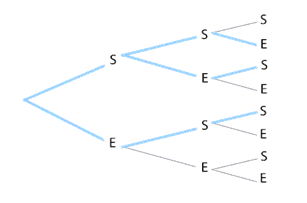
\includegraphics[width=0.75\textwidth,center]{coef_binomial.png}

chemin menant a k succes :\\ 
('SSS') k=3 ,('SSE') k=2 ,('SES') k=2,('SEE') k=1\\
('ESS') k=2 ,('ESE') k=1, ('EES') k=1,('EEE') k=0;\\
\\
-Pour k=0 , il y a 1 chemin qui mene a 0 succes , on note $(\limits^3_0)=1$\\
-Pour k=1 , il y a 3 chemins qui mene a 1 succes , $(\limits^3_1)=3$ \\
\\
Ou alors on peux utiliser la formule de la combinaisons $C\limits_3^1  \Leftrightarrow (\limits^3_1)=\frac{3!}{(3-1)!\times 1!}=\frac{1\times 2\times 3}{2!\times 1}=\frac{6}{(1\times 2)\times 1}=\frac{6}{2}=3$\\



\section{Permutation}
\underline{Utilité} : Avec n objets différents, combien de façons de les poser les uns à côté des autres?\\
\\
On peux represent\'e les permutation par un arbre pond\'er\'e avec autant de branche que poss\'ede l'ensemble
E .\\
\\
\underline{Formule} : n! \\
\\
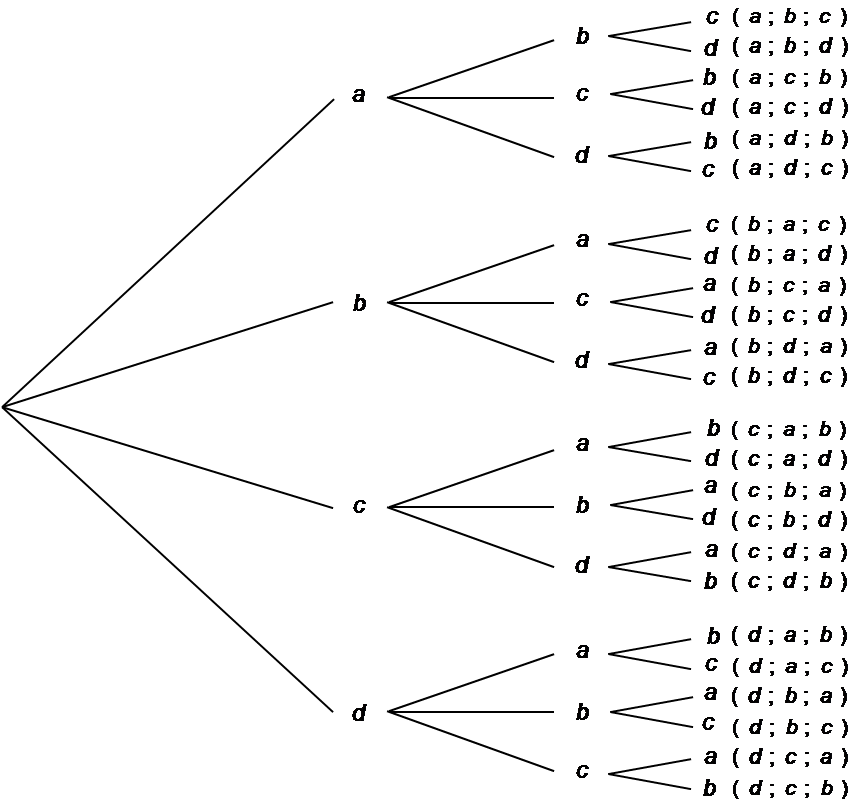
\includegraphics[width=0.75\textwidth,center]{permutation.png}
\\
Ici si on veux trouver tout les solution possible (permutation) de l'ensemble $card(\Omega) = 4 $ => {a,b,c,d} ou n=4 on a donc avec la formule : $n!=4!=4\times 3\times 2\times 1 = 24$. Il y a a bien 24 possibilités au totale .\\



\section{Arrangement}
\underline{Utilit\'e} :  Nous savons permuter  (mélanger) les cartes, maintenant nous en prenons quelques unes, l'une après l'autre, dans l'ordre. Nous nous retrouvons devant combien de possibilités? \\
\\
noté $A\limits_p^n$ , E etant un ensemble a n element .On appelle arrangement de p element de E toute p-liste d'éléments distinct de E.\\
\\
\underline{Formule} : $A\limits_n^p = \frac{n!}{(n-p)!}$\\ 
$A\limits_n^p$ peux s'ecrire ($\limits^n_p$) (p element parmie n)\\
\\
La probabilite qu'un evenement arrive peut changer selon leur ordre (ordonné/non-ordonné) et selon leur r\'ep\'etition (avec/sans r\'ep\'etition/remise) .Le fait d'avoir une factoriel dans la formule signifie en gros qu'il y a des permutation.  \\
\\

\section{Coeficient de correlation}

\underline{Utilité}:\\Le coefficient de corr\'elation lin\'eaire $r$ donne une mesure de l'intensit\'e et du sens de la relation lin\'eaire entre deux variables.\\
\\
-Le coefficient de corr\'elation est compris entre −1 et 1.\\
\\
-Plus le coefficient est proche de 1, plus la relation lin\'eaire positive entre les variables est forte.\\
Si $r=1$ la corr\'elation est positive parfaite.\\
\\
-Plus le coefficient est proche de −1,plus la relation lin\'eaire négative entre les variables est forte.\\
Si $r=-1$ la corr\'elation et=st negative parfaite.\\
\\
-Plus le coefficient est proche de 0, plus la relation lin\'eaire entre les variables est faible.\\
Si r=0 abscence totale de correlation.\\
\\
\textbf{Methode des moindre carr\'e} : \\
\\
\underline{Formule} : \\
-coef. corr\'elation $r=\frac{\sum(X-\overline{X}).(Y-\overline{Y})}{\sqrt{\sum(X-\overline{X})^2}\times (\sqrt{(Y-\overline{Y})})}$\\
\\
-Droite de regression : $Y=a.X.b$\\
-Pente(coef a) : $a=\frac{\sum(X-\overline{X}).(Y-\overline{Y})}{\sum(X-\overline{X})^2}$ 
$\left\{
\begin{array}{l}
  a>0 \text{correlation positive} \\
  a<0 \text{correlation negative} \\
  a=0 \text{pas de correlation}
\end{array}
\right.$
\\
Le point moyen est donnée en cordonne(\overline{X},\overline{Y}).\\

-Ordonnee a l'origine(coef b) : \overline{Y}-a.\overline{X}\\

%%%%%%%%%%%%%%%%%%%%%%%%%%%%%%%%%%%%%%%%%%%%%%%%%%%%%%%%%%%%%%%%%%%%%%%%%%%%%%%%%%%%%%%%%%%%%%%%%%%%%%%%%%%%

\chapter{Probabilit\'e}

\section{Calcule de probabilite}
Les probabilit\'é permete de decrire la possibilit\'e qu'un evenement particulier se produise dans un ensemble 
donn\'ee .La probabilité d'un événement est un nombre réel compris entre 0 et 1. Plus ce nombre est grand, plus le risque, ou la chance, que l'événement se produise est grand.Elle se note P(X=xi) \Rightarrow \text{probabilit\'e que la v.a X prenne la valeur xi}.\\
\\
\underline{Propriete} : \\
\\
- $P(\Omega)=1$\\
- $P(\overline{A})=1-P(A)$\\
\\
\underline{Exemple} :\\
\\
Un jeux 10 cartes , 6 noires et 4 rouges . on veux savoir la probabilite de tir\'e 2 cartes noires.\\
\\
-1er Carte noire : $P(X1= noir) = \frac{6}{10}$ \\
\\
-2ieme cartes noire : $P(X2= noir)= \frac{5}{9}$ on a enlever 1 noire il reste toujour 4 rouges .\\
\\
Les tirages sont \textbf{dependant} , le 2ieme tirage depant du 1er tirage.\\
\\
-$P(X = $2 noir$)=P(X1)+P(X2) =\frac{6}{10}\times \frac{5}{9}=\frac{30}{90}=\frac{1}{3}$\\
\\


\subsection{Probabilite conditionnel}
Ici ont a calculer des probabilite simple avec une seul condition , quand il y  plusieurs condition \\
$P_{b}(A)=$"tirer un 7 de trefle" avec P(A)="tirer un trefle" et P(B)="tirer un 7" , on appelle cela une \textbf{Probabilite Conditionnel}, elle se traduit par "probabilité de A sachant B".\\
\\
Elle se note $P_{b}(A)=P(A|B)=\frac{P(A\cap B)}{P(B)}$\\
\\
On dit que A et B sont incompatibles si et seulement si $A\cap B=\emptyset$\\
\\
$P(A \cup B)=P(A)+P(B)−P(A \cap B)$ \\
si A et B sont icompatibles la formule devient : $P(A \cup B)=P(A)+P(B)\\
\\
$P(A\cap B)=P(A)\times P(B)$ si A et B independant .\\




\section{Independance}
Quand il y a un tirage avec remise chaqu'un des resultat de l'arbre ne dependras pas du precedent , on dit que les experience sont identique et \textbf{independant}.\\
\\
\underline{Exemple}:\\
\\
On tire aux hasards une cartes dans un jeu de 32 cartes .\\
L'\'ev\'enement A:"Tirer un coeur" et B:"Tirer un roi".\\
Calculer $P(A)$ et $P_{b}(A)$ ? \\
\\
On est en situation d'\textbf{equiprobabilite} c-a-d que chaque tirage a la meme probabilite de tirage et 
$\Omega$ est l'ensemble des 32 cartes.\\
\\
\underline{Formule} : \\
$P(A)=\frac{card(A)}{card(\Omega)}$\\
\\
\text{Pour P(A) , sachant qu'il y a 8 coeur }:  $\frac{8}{32}=\frac{1}{4}$\\
Pour $P_B(A)=\frac{1}{4} \Rightarrow$ un roi parmie les coeurs.\\
Donc $P(A)=P_B(A)$ ,les evenement A et B sont independant.\\
\\
Ou alors avec cette formule : $P(A)\times P(B)=P(A\cap B)$\\
$P(A\cup B)=P(A)+P(B)-P(A\cap B)$\\
$P_B(A)=\frac{P(A\cap B)}{P(B)} \Rightarrow$ probabilite conditionnel\\
\\
$P(A)=\frac{1}{4} , P(B)=\frac{4}{32} \Leftrightarrow \frac{1}{8}$ , 
$P(A\cap B)=\frac{1}{4}\times \frac{1}{8}=\frac{1}{32}$\\
\\
\underline{Note} : \\
Si un evenement est dependant ont multiplie les probabilite , sinon si l'evenement est independant on additionne les probabilite .\\

\chapter{Variable Aleatoire}
\section{Variable Aleatoire Discret/Continue}
\subsection{Generalite}
\underline{Vocabulaire} :\\
\\
\textbf{Discret} : Cela veux dire que la variable aleatoire (v.a) X auras un nombre fini de valeurs dans un ensemble.\\
\\
\textbf{Continue} : Cela veux dire que la v.a X peux prendre n'importe quelle valeur dans un intervale. Soit X une v.a a valeurs dans R et fx une densite de probabilite sur R .On dit que X est une v.a continue de densite fx si pour tout intervalles A de R on a : P(X \in A)= $ \int_a^b f(x) \, \mathrm dx$\\
\\
\underline{Exemple}:\\
\\
Prenons une experience aleatoire d'un lanc\'e de 2 d\'es :\\
La variable aleatoire X auras comme valeur , $\Omega$={2,3,4,5,6,7,8,9,10,11,12} .La v.a X ne pourras prendre qu'une seule valeur parmie l'ensemble donc v.a discrete .
\\
Si par exemple on une intervalle d'heure d'arriver de maxime de 16h a 17h [16,17].\\
X la v.a qui indique l'heure d'arriver de maxime . X pourras prendre toute les valeurs compris dans l'intervalle [16,16.01,..,16.59,17] donc v.a continue .

\subsection{Determiner une loi de probabilite}
\underline{Probabilite Discrete}\\
\\
- Determiner la loi d'une  \textbf{probabilite discrete} :\\
1) Determiner l'ensemble des valeurs que peux prendre X .\\
2) Calculer P(X=$x_i$) pour chacune de ces valeurs $x_i$ .\\
\\
On peux representer graphiquement une loi de probilite discret avec un diagramme en baton .\\
\\
\underline{Probabilite Continue}\\
\\
- Determiner la loi d'une  \textbf{probabilite Continue} :\\
1) Calculer sa densite , La fonction de densit\'e se note pour $P(a\leq X\leg b)=\int_a^b f(x) \, \mathrm dx$\\
\\
On dit que la loi d'une variable continue en donnant la probabilite qu'elle appartiennent a un intervalles I quelconque .\\
Une v.a continue X , de densite fx, tombe entre a et b avec une probabilite egale a : $P(a \le X \le b)=\int_a^b f(x) \mathrm dx$ .\\
Plus la densite est elevee au dessus d'un segment , plus les chances que X a d'atteindre ce segment seras elevee , d'ou le terme "densite" .\\


\chapter{Loi de Probabilite}
\section{Loi d'une V.A Discrete}

\subsection{Loi Bernouilli}

Soit un univers constiue de deux eventualite S pour succes et E pour echec , $\Omega ={E,S}$ et se note B(1,p).\\
X($\Omega$)={0,1}.\\
La loi de probabilite associe a la variable de bernouilli tel que:\\
P(X=1)=p\\
P(X=0)=q avec p+q=1\\ 
avec p:probabilite que l'evenement soit vrais et q:probabilite inverse donc que l'evenement soit faux (1-p).\\
\\
\textbf{Esperance} : E(X)=p\\
\textbf{Variance} : V(X)=p(1-p)\\ 

\subsection{Loi Binomial}

La variable binomial Sn represente le nombre de succes obtenue lors de la repetition de n epreuve de bernouilli identitique et independante ,elle possede des valeurs discrete et se note B(n,p) avec n:nombre repetiton et p:probabilite de succes .\\
Sn = $\sum\limits_{i=1}^n$ Xi -> B(n,p) (signifie que la somme des proba de Sn suivent la loi binomial de parametre n,p). La loi binomial peux avoir 1 ou 2 parametre :\\
\\
-Binomial a 1 parametre B(p) pour k succes : \\
P(X=k)=$\left\{
\begin{array}{l}
  p \text{ si k}=1 \\
  1-p \text{ si k}=0
\end{array}
\right.$\\
\\
-Binomial a 2 parametres B(n,p) : \\
P(X=k)=$C_n^k.p^k.(1-p)^{n-k}$\\
\\
L'esperance et la variance ne change pas que ce soit le meme nombre de parametre ou non.\\
\\
\textbf{Esperance} : $E(X)=n\times p$\\
\\
\textbf{Variance} : V(X)=n.p.(1-p)\\ 

\subsection{Loi Poisson}
La loi Poisson est discrete, P(n,p) ou $P(\lambda)$ , permet de faire une approximation de la loi binomial pour rendre les mesures plus prescise .On utilise cette approximationn de loi lorsque un grand nombre d'evenement qui suivent la loi binomial et qu'on connait la moyenne $\lambda , n\geq 100$ et $n\times p\leq 10$.\\
\\
\underline{Formule} :  $X->P(\lambda) \tab P(X=k)=e^{-\lambda}.\frac{\lambda^k}{k!}$ avec $\lambda=n\times p$\\
\\

\subsection{Loi Uniforme}
\textbf{V.A Discrete}
La loi Uniforme discrete sur un ensemble fini est la loi des "tirages au hasard" dans cet ensemble ou il y a equiprobabilite.
Une distribution de probabilite suit une lois Uniforme lorsque les valeurs prises par la va. sont equiprobable.
$\forall i , P(X=xi) = \frac{1}{n}$ avec n:nombre de valeur different que prend la v.a X donc cardinal .\\
Par exemple pour un lanc\'e de d\'e on auras une probabilite de $\frac{1}{6}$ de tir\'e  pour chacune des faces du d\'e .\\
\\
\underline{Formule} : X -> U(En) \\
P(X=k)=$\frac{1}{n}$ \\

\begin{center}
\begin{tabular}{|c|c|c|c|c|c|}
\hline
P(X=1) & P(X=2) & P(X=3) & P(X=4) & P(X=5) & P(X=6) \\ \hline
$\frac{1}{6}$ & $\frac{1}{6}$ & $\frac{1}{6}$ & $\frac{1}{6}$ & $\frac{1}{6}$ & $\frac{1}{6}$ \\ \hline
\end{tabular}
\end{center}

\textbf{Esperance} : $E(X)=\sum\limits_{i=1}^{i=n} xi.pi$ avec xi:numeros de repetition (i a n) 
et pi:peux s'ecrire P(X=xi\\
\\
\textbf{Variance} : $V(X)=\sum\limits_{i=r}^{i=n}(xi-E(x))^2.pi$ ou ou $V(x)=(\sum\limits_{i=1}^n xi^2 .pi$ ou $V(X)=\frac{n^2-1}{2}$\\
\\

\section{Loi d'une V.A Continue}

\subsection{Loi Uniforme}
\textbf{V.A continue}\\
\\
\underline{Fonction de densit\'e} : f(x)= $\left\{
\begin{array}{l}
  \frac{1}{b-a} \text{ si x} \in \text{[a;b]} \\
  0 \text{ sinon}
\end{array}
\right.$\\
\\
Les valeurs de la v.a X correspond au rang xi=i ,($\forall i \in$ [1,n]). on a :\\
\\
\textbf{Variance} : E(X)=$\frac{b+a}{2}$ \\
\textbf{Esperance} : V(x)=$\frac{(b-a)^2}{12}$\\

\subsection{Loi Normale}
La loi normale est continue est permet de faire une approximation de la loi binomial.On l'utilise lorsque , n est assez grand et p pas trop proche de 0 ou 1 .\\
\\
\underline{Fonction de densite} : $f(x)=\frac{1}{\sigma\sqrt{2\pi}}e^{-\frac{(x-\mu)^2}{2\sigma^2}}$
\\
\underline{Formule} :  X->N(np,np(1-p)) ou $X->N(\mu,\sigma)$\\
\\\textbf{Esperance} : $E(X)= \mu $\\
\\
\textbf{Variance} : $V(X)=\sigma^2$

\end{document}